\documentclass[a4paper, 14pt, oneside]{article}

% \setcounter{secnumdepth}{0}
\usepackage{sectsty}

\chapternumberfont{\fontsize{14}{14}\selectfont} 
\chaptertitlefont{\fontsize{14}{14}\selectfont}
\sectionfont{\fontsize{14}{14}\selectfont}
\subsectionfont{\fontsize{14}{14}\selectfont}

%% подключаем стандарт библиографии
\bibliographystyle{gost71u} 

%% for envirovemt "abstract" in class book
% \newenvironment{abstract}{}{}
% \usepackage{abstract}

%% подключаем преамбулу, в ней содержатся подключение всех необходимых пакетов
%%% Работа с русским языком
\usepackage{cmap}			 % поиск в PDF
\usepackage{mathtext} 		 % русские буквы в формулах
\usepackage[T2A]{fontenc}	 % кодировка
\usepackage[utf8]{inputenc}	 % кодировка исходного текста
\usepackage[russian]{babel}	 % локализация и переносы

%%% Пакеты для работы с математикой
\usepackage{amsmath,amsfonts,amssymb,amsthm,mathtools}
\usepackage{icomma}

%% Номера формул
%\mathtoolsset{showonlyrefs=true} % Показывать номера только у тех формул, на которые есть \eqref{} в тексте.
%\usepackage{leqno}               % Немуреация формул слева

%% Шрифты
\usepackage{euscript}	 % Шрифт Евклид
\usepackage{mathrsfs}    % Красивый матшрифт

%% Поля (геометрия страницы)
\usepackage[left=3cm,right=1.5cm,top=2cm,bottom=2cm,bindingoffset=0cm]{geometry}

%% Русские списки
\usepackage{enumitem}
\makeatletter
\AddEnumerateCounter{\asbuk}{\russian@alph}{щ}
\makeatother

%%% Работа с картинками
\usepackage{caption}
\captionsetup{justification=centering} % центрирование подписей к картинкам
\usepackage{graphicx}                  % Для вставки рисунков
\graphicspath{{images/}{images2/}}     % папки с картинками
\setlength\fboxsep{3pt}                % Отступ рамки \fbox{} от рисунка
\setlength\fboxrule{1pt}               % Толщина линий рамки \fbox{}
\usepackage{wrapfig}                   % Обтекание рисунков и таблиц текстом

%%% Работа с таблицами
\usepackage{array,tabularx,tabulary,booktabs} % Дополнительная работа с таблицами
\usepackage{longtable}                        % Длинные таблицы
\usepackage{multirow}                         % Слияние строк в таблице

%% Красная строка
\setlength{\parindent}{1.25cm}

%% Интервалы
\linespread{1.3}
\usepackage{multirow}
\usepackage{indentfirst}
\usepackage[14pt]{extsizes}

%% TikZ
\usepackage{tikz}
\usetikzlibrary{graphs,graphs.standard}

% %% Верхний колонтитул
\usepackage{fancyhdr}
\pagestyle{fancy}

%% Перенос знаков в формулах (по Львовскому)
\newcommand*{\hm}[1]{#1\nobreak\discretionary{}{\hbox{$\mathsurround=0pt #1$}}{}}

%% дополнения
\usepackage{float}   % Добавляет возможность работы с командой [H] которая улучшает расположение на странице
\usepackage{gensymb} % Красивые градусы
\usepackage{caption} % Пакет для подписей к рисункам, в частности, для работы caption*

% подключаем hyperref (для ссылок внутри  pdf)
\usepackage[unicode, pdftex]{hyperref}


\usepackage[backend=biber]{biblatex}
\addbibresource{references.bib}

\geometry{
    a4paper,
    left=30mm,
    right=15mm,
    top=20mm,
    bottom=20mm,
    bindingoffset=0cm
}

\begin{document}
%% титульник
% \begin{center}
    %% *название института*
    \large\textbf{Министерство образования и науки Российской Федерации \\
        Московский физико-технический институт (государственный
        университет)} \\
    \vspace{1cm}

    %% *факультет/физтех-школа*
    Физтех-школа радиотехники и компьютерных технологий \\

    %% *название базовой кафедры и лаборатории*
    %% в случае ненадобности можно удалить
    Кафедра микропроцессорных технологий в интеллектуальных системах управления \\
    % Лаборатория (laboratory name)\\

    \vspace{3em}

    Выпускная квалификационная работа бакалавра
\end{center}

\begin{center}
    \vspace{\fill}
    %% *название вашей работы*
    \LARGE{Применение методов машинного обучения в статистическом анализе}

    \vspace{\fill}
\end{center}


\begin{flushright}
    \textbf{Автор:} \\
    Студент Б01-818 группы \\
    Назаров Константин Олегович \\
    \vspace{2em}
    \textbf{Научный руководитель:} \\
    Гаврин Евгений Александрович  \\
\end{flushright}

\vspace{7em}

\begin{center}
    %% *лого*
    
\includegraphics[width=100 pt]{MIPT_logo.jpg}\\
    Москва \the\year{}
\end{center}

% выключаем отображение номера для этой страницы (титульник)
\thispagestyle{empty}

\newpage
\setcounter{page}{2}
\fancyfoot[c]{\thepage}
% *надпись над верхним колонтинулом*
% в случае ненадобности можно удалить
\fancyhead[L]{Применение методов машинного обучения в статистическом анализе}
\fancyhead[R]{}
%% аннотоция
\begin{abstract}

    \begin{center}
        \large{Применение методов машинного обучения в статистическом анализе} \\
        \large\textit{Назаров Константин Олегович} \\[1 cm]
    \end{center}


    Статические анализаторы широко используются в промышленности для нахождения и исправления уязвимостей в коде в процессе разработки, тем самым улучшая качество кода и упрощая дальнейшую разработку. Однако их применение ограничивается тем, что на больших и сложных кодовых базах статические анализаторы выдают большое количество false positives наряду с предупреждениями о действительных уязвимостях. Поэтому значительная часть данной работы посвящена тому, чтобы применить методы машинного обучения для классификации и приоритизации сообщений статического анализатора, что позволит сократить время, затрачиваемое разработчиками на ручную обработку всех сообщений анализатора. Основной проблемой при обучении подобного классификатора является составление тренировочного датасета, т.к. неочевиден алгоритм разметки данных и признаки для обучающей выборки. Также большим фактором является скрость генерации: признаки не должны вычисляться долго, т.к. сам статический анализ занимает очень большое время (для относительно простых анализаторов время работы примерно в 2 раза превышает время компиляции, но может быть и много больше \cite{GCC-SA}). В данной работе рассматривается способ генерации датасета при помощи тестовых сюит для статических анализаторов (т.е. репозиториев с "образцовыми" программами, специально написанными для тестирования статических анализторов), а также показывается, что включение в обучающий датасет token-based представления кода помогает увеличить способность к распознаванию разных шаблонов ошибок, не увеличивая при этом сложности генерации датасета. Данные для обучения были получены путем применения нескольких статических анализаторов к кодовой базе Juliet C/C++ Test Suite v1.3. Разметка была произведена автоматически из метаданных тестовой сюиты. Полученный датасет был использован для обучения двух моделей: decision tree и gradient boosting, предоставляемых библиотекой xgboost для python3. Полученные классификаторы имеют высокую точность на тестовой выборке ($\approx 96~\%$). Также в работе был предложен альтернативный метод генерации датасета, призванный решить проблемы использованного метода. Применение альтернативного метода является предметом дальнейших исследований.

    \vfill

\end{abstract}

%содержание
\tableofcontents{}
\newpage

\chapter{Введение}
\label{sec:Chapter0} \index{Chapter0}

\subsection*{Обозначения и сокращения}

\begin{enumerate}
    \item False Positive, FP - ошибка бинарной классификации, при которой классификатор ошибочно предсказывает положительный результат (например диагноз болен, когда болезни на самом деле нет)
    \item Датасет - это обработанная и структурированная информация в табличном виде. Строки такой таблицы называются объектами, а столбцы – признаками (фичами)
    \item Token-Based представление - представление кода в виде последовательности токенов, получаемых в результате лексического анализа
    \item Тестовая сюита - специализированный набор тестов
    \item Abstract Syntax Tree, AST - представлнение исходного кода в виде дерева абстрактного синтаксиса
    \item Application Programming Interface, API - описание способов (набор классов, процедур, функций, структур или констант), которыми одна компьютерная программа может взаимодействовать с другой программой
    \item Common Weakness Enumeration, CWE \cite{CWE-doc} - Список уязвимостей программного и аппаратного обеспечения. Является общепринятым языком для описания природы уязвимости
    \item NIST - The National Institute of Standards and Technology
    \item SATE - Static Analysis Tool Expositions
\end{enumerate}

\subsection*{Введение}

Статические анализаторы широко используются в промышленности для нахождения и исправления уязвимостей в коде в процессе разработки, тем самым улучшая качество кода и упрощая дальнейшую разработку. Однако их применение ограничивается Множеством факторов. Статья "A Few Billion Lines of Code Later. Using Static Analysis to Find Bugs in the Real World"\cite{Bessey2010AFB} раскрывает множество проблем с применением статических анализаторов на практике, среди которых: большое количество false positives ($35\% - 91\%$ \cite{HECKMAN2011363})  на сложных или больших кодовых базах; пользователи, помечающие непонятные им сообщения как ложные; а также сложность обработки большого количества ошибок пользователем, которая приводит к тому, что анализаторы выдают меньше сообщений, чем могли бы. В связи с этим, Moritz Marc Beller с коллегами \cite{Beller2016AnalyzingTS} обнаружили, что на практике очень малое число проектов с открытыми исходным кодом интегрирует статические анализаторы в процесс разработки. Также большая часть проектов не поддерживается правила, что предупреждения компиляции должны рассматриваться как ошибки.  Поэтому значительная часть данной работы посвящена тому, чтобы применить методы машинного обучения для классификации и приоритизации сообщений статического анализатора, что позволит сократить время, затрачиваемое разработчиками на ручную обработку всех сообщений анализатора а также облегчит эффективное использование анализаторов на практике. Основной проблемой при обучении подобного классификатора является составление тренировочного датасета, т.к. неочевиден алгоритм разметки данных и признаки для обучающей выборки. Также большим фактором является скорость генерации: признаки не должны вычисляться долго, т.к. сам статический анализ занимает очень большое время (для относительно простых анализаторов время работы примерно в 2 раза превышает время компиляции, но может быть и много больше \cite{GCC-SA}). В промышленности эта проблема решается тем, что датасет зачастую имеется\cite{Ruthruff2018PredictingAA} \cite{classification-models-multiple-SA-tools} или может быть легко получен из статистики использования или из истории проекта\cite{assesing-validity-of-sa-warnings-cisco}. В данной работе рассматривается способ генерации датасета при помощи тестовых сюит для статических анализаторов\cite{test-suites-for-dataset} (т.е. репозиториев с "образцовыми" программами, специально написанными для тестирования статических анализаторов), а также показывается, что включение в обучающий датасет token-based представления кода помогает увеличить способность к распознаванию разных шаблонов ошибок, не увеличивая при этом сложности генерации датасета. Данные для обучения были получены путем применения нескольких статических анализаторов к кодовой базе Juliet C/C++ Test Suite \cite{Juliet}. Разметка была произведена автоматически из метаданных тестовой сюиты. Полученный датасет был использован для обучения двух моделей, которые впоследствии были протестированы на тестовой выборке.

\newpage %% Введение
\chapter{Постановка задачи}
\label{sec:Chapter1} \index{Chapter1}

Основной целью данной работы является сокращение времени, затрачиваемого разработчиком на обработку результатов статического анализа. Также важной целью является применение полученных результатов для анализа работы статического анализатора и его дальнейшей настройки. Для достижения обозначенной цели требуется решить следующие задачи:

\begin{enumerate}
    \item Определить признаки для будущего датасета.
    \item Определить метод генерации датасета и его разметки. Собрать данные.
    \item Обучить классификатор сообщений статического анализатора.
    \item Проанализировать полученные результаты.
\end{enumerate}

Для того, чтобы результат работы считался удовлетворительным и применимым на больших масштабах, решения для поставленных задачи должны удовлетворять следующим требованиям:

\begin{enumerate}
    \item Сложность извлечения признаков не должна превосходить сложности статического анализа.
    \item Разметка датасета должна быть автоматизированной, т.к. ручная разметка занимает слишком долгое время и требует наличия проанализированной большой кодовой базы \cite{Ayewah2010TheGF}.
    \item Классификатор не должен быть ограничен конкретными анализаторами, т.е. должен иметь возможность обработать и классифицировать предупреждение от любого анализатора после необходимой обработки.
\end{enumerate}

\newpage %% Постановка задачи
\section{Обзор существующих решений и литературы}
\label{sec:Chapter2} \index{Chapter2}

Необходимость поддержки множества анализаторов обуславливается еще и тем, что каждый анализатор покрывает лишь конечное число уязвимостей, упуская остальные\cite{Delaitre2013OfMS, 3291, Bessey2010AFB}. Поэтому для получения наиболее полного по типам ошибок датасета необходимо уметь обрабатывать сообщения от разных анализаторов. Решением данной проблемы является приведение всех кодов ошибок к кодам CWE \cite{CWE-doc} на этапе обработки сообщения и использование соответствующего кода CWE в датасете при обучении и классификации. Таким образом, добавление поддержки нового анализатора заключается в трансляции кода ошибок анализатора в CWE. Более подробно данный метод будет описан в дальнейшем в соответствующем разделе \ref{sec:Err-to-CWE}.

Sarah Heckman и Laurie Williams в своем исследовании\cite{HECKMAN2011363} выделили следующие признаки, используемые в наиболее релевантных работах о классификаторах, подобных тому, который является целью данного диплома:
\begin{enumerate}
    \item Характеристики ошибки - атрибуты предупреждения, сгенерированного статистиким анализатором, например: тип ошибки (double free, etc.), местоположение в коде (файл, класс, функция, строка, etc.), а также приоритет, который анализатор присвоил ошибке.
    \item Характеристики кода - метрики кода, в котором содержится предупреждение. Эти метрики могут быть извлечены при помощи дополнительного анализа или из самого кода (цикломатическая сложность, количество строк в файле, etc.).
    \item Метрики репозитория с исходным кодом - атрибуты репозитория с исходным кодом (история коммитов, частота изменения кода, история ревью, etc.)
    \item Метрики базы данных с уязвимостями - информация об известных уязвимостях может быть связана с изменениями в исходном коде для того, чтобы идентифицировать уязвимость и необходимые исправления.
    \item Метрики динамического анализа - гибридное использование статического и динамического анализа может помочь устранить затраты, связанные с исполнением каждой техники анализа.
\end{enumerate}

В данной работе внимание было сосредоточено целиком на первых двух пунктах: характеристики ошибки и характеристики кода. Изучив соответствующие статьи, было выяснено, что основными характеристиками кода для последующего анализа являются метрики, такие как число вложенности функции, число условных переходов, цикломатическая сложность, etc \cite{test-suites-for-dataset}. Однако все эти метрики являются метаданными, которые лишь характеризуют код в целом, не давая понятия о его структуре. Для того, чтобы каким либо образом анализировать структуру кода обычно используется представление AST\cite{Shedko2020ApplyingPM}. Такой подход хорош для таких языков как Java, Python, где AST может быть легко получено. Для получения же AST в C/C++ необходима полная компиляция проекта. Т.к. каждый проект имеет свои систему для сборки, то невозможно описать данную процедуру единым простым путем. Поэтому в данной работе был опробован подход на основе token-based представления кода, предложенного в \cite{Shedko2020ApplyingPM} для задач определения стиля проекта и вывода правил использования API. Идея состоит в том, что хоть представление в виде токенов и является неточным, но отфильтровав его, и анализируя наряду с метаданными кода, может быть получена более полная картина, нежели чем при использовании только метаданных. Включение токенов в обучающую выборку производилось в предположении, что все false positives следуют определенным шаблонам, которые могут быть определены при помощи предварительно обработанного token-based представления кода. Данное предположение было подробно изучено в работе Zachary P. Reynolds\cite{Reynolds}, в которой была произведена классификация этих шаблонов для нескольких статических анализаторов. Более подробно о token-based представлении в качестве признаков будет рассказано в соответствующем разделе \ref{Tokens}.

В большинстве рассмотренных работ для классификации используются либо решающие деревья, либо LSTM нейронные сети\cite{test-suites-for-dataset, assesing-validity-of-sa-warnings-cisco}. В данной работе будет рассмотрен только классификатор на основе решающих деревьев, и решения на основе рекуррентных нейронных сетей являются предметом дальнейших исследований, т.к. могут помочь находить более сложные шаблоны ошибок.

Для разметки датасета предлагаются разные способы. Anshul Tanwar с коллегами в своей работе \cite{assesing-validity-of-sa-warnings-cisco} предлагают способ разметки false positive на основе истории коммитов репозитория. В своей статье авторы брали исправления разработчиков в течение жизни проекта и сопоставляли их с отчетами статического анализатора. После чего производилась разметка: если исправление касалось куска кода, в котором анализатор находил уязвимость, то ставилась метка true positive, то есть верное предсказание. Иначе, если разраобтчик помечал данный кусок кода как безопасный, то сообщение анализатора помечалось как false positive. Этот подход обладаем многими преимуществами, такими как больший охват различных сценариев срабатывания анализатора, то есть обученный на подобных данных классификатор будет более гибким, т.к. запомнит более реалистичные шаблоны, нежели классификатор, обученный на рукописных тестах. Также преимуществом данного подхода является относительная простота реализации. Данный подход имеет несколько минусов. Первый - это необходимость наличия сторого формализованной истории коммитов в репозитории, чтобы суметь эффективно извлечь информацию об исправлениях. Второй - необходимость наличия сообщений, помеченных разработчиками как false positive, что возможно только при должном уровне интеграции статического анализа в процесс разработки, что, как показал предыдущий анализ литературы, является большой редкостью. Третий - необходимость запускать анализ проекта много раз на разных этапах жизни для корректной разметки, что является очень ресурсоемким и долгим процессом. Другой подход, предложенный в работе Lori Flynn с коллегами \cite{test-suites-for-dataset}, избегает многих минусов первого подхода за счет уменьшения охвата кодовой базы. В этой статье авторы использовали Juliet Test Suite - набор рукописных тестов, предназначенных для валидации эффективности различных статистиких анализаторов\cite{Juliet} для составления и разметки своего датасета. Подход к генерации датасета, используемый в данной работе был позаимствован из этой работы.

\newpage %% Обзор существующих решений
\section{Построение решений задач}
\label{sec:Chapter3} \index{Chapter3}

После анализа литературы и уже существующих решений стало ясно, как реализовывать каждую из поставленных ранее задач. Далее будет рассказано о том, какие методы были выбраны для выполнения этих задач. Порядок, в котором они были объявлены в разделе \ref{sec:Chapter1} сохранен.

\subsection{Признаки для датасета}
\label{sec:dataset} \index{dataset}

Обсудим признаки, которые были выбраны для обучения классификатора. В предыдущем разделе \ref{sec:Chapter2} было сказано, что из всех признаков, указанных в \cite{HECKMAN2011363}, данная работа сфокусируется лишь на первых двух - характеристики ошибки и характеристики кода, опуская последние три - метрики репозитория с исходным кодом, метрики базы данных с багами, метрики динамического анализа. Далее будет описано, почему при составлении датасета был опущен каждый из перечисленных классов признаков, а также будет описано то, какие признаки все же были представлены в датасете в настоящей работе.

\subsubsection{Метрики репозитория с исходным кодом}
Как было обозначено в обзоре литературы \ref{sec:Chapter2}, для того, чтобы хоть сколько нибудь эффективно анализировать историю коммитов проекта, она должна быть строго организована, иначе поиск нужных мест в коде сводится к полному анализу всего проекта на каждом из этапов его разработки. В том же разделе было объяснено, что в открытом доступе очень малое число проектов соблюдает подобные правила. Плюс, даже при их соблюдении, множественный анализ проекта очень дорог вычислительно и по времени. Плюс, для того, чтобы размечать false positives, необходимо иметь доступ к уже собранной статистике использования анализатора, которой не существует в открытом доступе. Таким образом, анализ истории коммитов и других метрик репозитория отпадает.

\subsubsection{Метрики базы данных с уязвимостями}
Как и в предыдущем пункте, применение данных метрик ограничивается их отсутствием в открытом доступе.

\subsubsection{Метрики динамического анализа}
Для проведения динамического анализа требуется полная сборка всего проекта, что добавляет сложности к и без того затратному процессу анализа. Также, основным предметом изучения данной работы является именно статический анализ, поэтому рассмотрение метрик динамического анализа было решено оставить как предмет для будущих исследований.

\subsubsection{Характеристики ошибки}
\label{sec:Err-to-CWE} \index{Err-to-CWE}
Для того, чтобы удовлетворить требованию языковой независимости, все сообщения анализаторов требуется приводить к общему виду. Таким общим видом было выбрано представление Common Weakness Enumeration (CWE)\cite{CWE-doc}. Таким образом, добавление нового статического анализатора к списку поддерживаемых сводится к добавлению интерфейса, транслирующего код ошибки анализатора в код CWE. К счастью, для большинства распространенных статических анализаторов существуют таблицы соответствия или настройки, позволяющие выводить код ошибки сразу в формате CWE.

\subsubsection{Характеристики кода}
В проанализированной литературе основными признаками, по которым производилось обучение, являлись метрики кода. Чаще всего речь шла о метриках таких как вложенность, цикломатическая сложность, количество путей через выделенный фрагмент кода, etc. В данной работе метрики кода считались только для функции, в которой анализатор обнаружил уязвимость. Замеры производились при помощи утилиты ccsm\cite{CCSM}, в которую были дополнительно внесены изменения. Реализована данная утилита как инструмент в инфраструктуре Clang\cite{Clang}. Этот инструмент вызывает парсер Clang для указанного файла, и работает с полученным частичным промежуточным представлением. Т.к. полная компиляция проекта не требуется (парсинг производится лишь на выбранном файле), то извлечение этих метрик не сказывается на общем времени сбора датасета. Метрики кода, использованные для обучения моделей в данной работе можно разделить на следующие группы:

\begin{enumerate}
    \item Количество ключевых слов, контролирующих поток исполнения программы (for, if, else, etc.)
    \item Различные способы подсчета цикломатической сложности
    \item Количество различных обращений к памяти (разименование указателя, обращение к полю, обращение к полю по указателю, etc.)
    \item Характеристики самой функции (количество путей через нее, вложенность)
\end{enumerate}

\subsubsection{Token-based представление кода}
\label{Tokens} \index{Tokens}
Описанные выше метрики характеризуют код лишь косвенно, не давая представления о его структуре. Таким образом теряется способность классификатора распознавать шаблоны, которые приводят к false positive. Чтобы бороться с этой проблемой был предложен подход на основе токенов. Токены были выбраны, т.к. анализ AST является затруднительным и более затратным. Токены, с другой стороны, можно получить еще на этапе лексического анализа. Вывод токенов был также реализован в качестве инструмента для Clang. Чтобы увеличить шансы на распознавание шаблонов false positive, представление кода в виде токенов было предварительно обработано: были оставлены только ключевые слова, влияющие на поток исполнения, операторы и идентификаторы.

\begin{figure}[H]
    \centering
    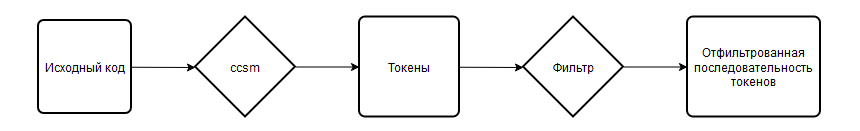
\includegraphics[width=\textwidth]{flow.png}
    \caption{Шаги получения отфильтрованной последовательности токенов}
\end{figure}

После предварительной обработки, из получившейся последовательности токенов выбирается подпоследовательность фиксированной длины, такая, что токен, на который указывает сообщение об ошибке находится ровно посередине подпоследовательности. Получившаяся подпоследовательность фиксированной длины называется окном и контролируется гиперпараметром WINDOW\_SIZE, отвечающим за ширину этого окна. Соответственно, в датасете появляются признаки token[0], token[1], token[2], ... token[WINDOW\_SIZE - 1]. Предположение данной работы состоит в том, что последовательности отфильтрованных токенов наряду с метаданными о коде должно хватить для распознавания большинства шаблонов false positive, указанных в \cite{Reynolds}.
\\
\\
Резюмируя, датасет, используемый для обучения моделей в данной работе, имеет следующий вид:

\begin{table}[H]
    \centering
    \resizebox{\textwidth}{!}{
        \begin{tabular}{|c|c|c|c|c|c||c|}
            \hline
            код CWE & token[0] & token[1] & ... & token[WINDOW\_SIZE - 1] & метрики кода & метка класса \\ \hline
        \end{tabular}
    }
    \caption{Общий вид элемента датасета}
\end{table}

\subsection{Метод генерации и разметки датасета}
Для генерации и разметки датасета была выбрана кодовая база Juliet Test Suite\cite{Juliet}. Имеющиеся в коде метаданные позволяют без проблем классифицировать большинство сообщений анализатора как false positive или true positive. Рассмотрим пример кода Juliet Test Suite:

\begin{verbatim}
    // CWE415_Double_Free__malloc_free_char_08.c
    ...
    void CWE415_Double_Free__malloc_free_char_08_bad()
    {
        ...
    }
    ...

    // manifest.xml
    ...
    <testcase>
      <file path="CWE415_Double_Free__malloc_free_char_08.c">
        <flaw line="47" name="CWE-415: Double Free"/>
      </file>
    </testcase>
    ...
\end{verbatim}

Juliet Test Suite содержит два типа метаданных, которые полезны при оценке верности предупреждений анализатора:
\begin{enumerate}
    \item manifest.xml - этот файл содержит точную информацию о каждой ошибке, включая номер строки, файл и тип ошибки.
    \item Названия функций - в документации к тестовой сюите говорится, что если название функции содержит строку 'GOOD', то указанный тип CWE в данной функции не встречается, а если название функции содержит строку 'BAD', то данный CWE в этой функции присутствует.
\end{enumerate}

Для разметки датасета были собраны следующие данные: для каждого файла, в котором анализаторы находили уязвимости были собраны метрики кода, а также token-based представление для каждой из функций. Далее стоит учитывать, что Juliet Test Suite указывает только на наличие или отсутствие конкретного CWE, указанного в названии файла, тоесть мы не можем выносить суждение о других типах уязвимостей, о которых сообщил анализатор в данном файле. Иными словами, если уязвимость, найденная анализатором не совпадает с CWE, указанным в manifest.xml или названии файла, то метаданные не могут быть использованы для того, чтобы пометить данное сообщение анализатора как true positive / false positive. Таким образом, после того, как вся тестовая сюита была проанализирована несколькими анализаторами, их сообщения об уязвимостях были слиты в единую базу данных, где каждый код ошибки был предварительно заменен на эквивалентный CWE либо при помощи встроенных в анализатор средств, либо при помощи уже заранее составленных таблиц соответствия. Далее, для каждого сообщения об ошибке была получена метка класса. Разметка происходила следующим образом:

\begin{enumerate}
    \item Если информация об уязвимости в manifest.xml (путь, строка, тип) совпадает с той, которую сообщил анализатор, то ставилась метка true positive
    \item Если уязвимость обнаружена в строках, принадлежащих функции с именем 'GOOD', и код ошибки совпадает с CWE, указанным в имени файла, то ставилась метка false positive.
\end{enumerate}

Для остальных случаев невозможно точно определить метку. Однако существуют спекулятивные методы, которые являются предметом для дальнейших исследований и не были рассмотрены в данной работе. Их применение позволит расширить кодовую базу, на которой обучается классификатор, что увеличит качество и количество распознаваемых шаблонов false positive.

Тестовая выборка была получена путем разбиения всего датасета в соотношении $30:70$, с сохранением этих пропорций для каждого из классов true positive и false positive.

\subsection{Обучение классификатора}

Выше было введено понятие обучения классификатора на размеченном датасете. Далее будут пояснены все использованные выше термины, такие как датасет, а также будут объяснены детали каждой из используемых моделей.

\subsection{Обучение с учителем}

Задачей машинного обучения является поиск функции, максимально приближающей заданную зависимость между элементами множества $X$ (объектами) и элементами множества $Y$ (таргетами), т.е. поиск $f(X):$
\[f(X) = Y + \varepsilon\]
где $\varepsilon$ - случайная величина, ошибка предсказания

Функция $f(X)$, отображающая объекты в таргеты, именуется моделью, а имеющийся у нас набор объектов иногда ещё называют обучающей выборкой или датасетом. Датасет состоит из:

\begin{enumerate}
    \item Объекты (признаки) - элементы множества X
    \item Метки (таргеты) - правильные ответы для $f(X)$.
\end{enumerate}

В обучении с учителем мы хотим при помощи обучающей выборки построить модель, предсказания которой достаточно хороши. Обычно, качество предсказаний измеряют с помощью метрик качества, то есть функций, которые показывают, насколько сильно полученные предсказания, выдаваемые моделью, похожи на правильные ответы. Цель обучения обычно состоит в том, чтобы получить как можно более лучшее (наибольшее или наименьшее возможное, в зависимости от ситуации) значение метрики.

Выделяют два основных типа задач обучения с учителем в зависимости от того, каким может быть множество $Y$ всех возможных ответов (таргетов):

\begin{enumerate}
    \item Регрессия - $Y \in \mathbb{R}$ или $Y \in \mathbb{R}^M$. Примерами задач регрессии является предсказание погоды на завтра (температуры, влажности, давления).
    \item Классификация - $Y = \{1,...,K\}$. Предсказание принадлежности объекта к одному из $K$ классов. В случае $K = 2$ данная задача называется бинарная классификация. Именно эта задача и решается в данной работе. Необходимо определить, является ли объект (уязвимость, предсказанная анализатором и ее описание, как описано выше в \ref{sec:dataset}) элементом класса false positive или true positive.
\end{enumerate}

\subsubsection{Решающее дерево. Decision tree}
Одной из самых простых, но при этом эффективных для хорошо отделимых классов, моделей для решения задачи бинарной классификации является решающее дерево. Это такое бинарное дерево, в котором:
\begin{enumerate}
    \item Каждой внутренней вершине $v$ приписан предикат $B_v: X \rightarrow {0, 1}$.
    \item каждой листовой вершине $v$ приписан прогноз $c_v \in Y$, где $Y$ — область значений целевой переменной (в случае классификации листу может быть также приписан вектор вероятностей классов).
\end{enumerate}

В ходе предсказания осуществляется проход по этому дереву к некоторому листу. Для каждого объекта выборки x движение начинается из корня. В очередной внутренней вершине $v$ проход продолжится вправо, если $B_v(x)=1$, и влево, если $B_v(x)=0$. Проход продолжается до момента, пока не будет достигнут некоторый лист, и ответом алгоритма на объекте $x$ считается прогноз $c_v$, приписанный этому листу\cite{SHAD-trees}.

Предикат $B_v$ может иметь, вообще говоря, произвольную структуру, но, как правило, на практике используют просто сравнение с порогом $t \in \mathbb{R}$ по какому-то $j$-му признаку:

\[ B_v(x,j,t)=[x_j \leq t] \]

При проходе через узел дерева с данным предикатом объекты будут отправлены в правое поддерево, если значение $j$-го признака у них меньше либо равно $t$, и в левое, если больше. В дальнейшем рассказе мы будем по умолчанию использовать именно такие предикаты.

Из структуры дерева решений следует несколько интересных свойств:\cite{SHAD-trees}

\begin{enumerate}
    \item Выученная функция является кусочно-постоянной, из-за чего производная равна нулю везде, где задана. Следовательно, о градиентных методах при поиске оптимального решения можно забыть.
    \item Решающее дерево (в отличие от, например, линейной модели) не сможет экстраполировать зависимости за границы области значений обучающей выборки.
    \item Решающее дерево способно идеально приблизить обучающую выборку и ничего не выучить (тоесть такой классификатор будет обладать низкой обобщающей способностью): для этого достаточно построить такое дерево, в каждый лист которого будет попадать только один объект. Следовательно, при обучении нам надо не просто приближать обучающую выборку как можно лучше, но и стремиться оставлять дерево как можно более простым, чтобы результат обладал хорошей обобщающей способностью.
\end{enumerate}

Теперь разберемся с тем, как построить дерево. Другими словами, обучить модель. Построение дерева будем рассматривать итеративно. Пусть $X$ - исходное множество объектов обучающей выборки, а $X_m$ - множество объектов, попавших в текущий лист (в самом начале $X_m = X$). Тогда алгоритм можно описать следующим образом:

\begin{enumerate}
    \item Рассмотрим вершину $v$. Если выполнен критерий остановки (например глубина дерева или степень ветвления), то останавливаемся, объявляем эту вершину листом и ставим ей в соответствие ответ.
    \item Иначе, находим предикат $B_{j,t}$, который даст наилучшее разбиение текущего множества $X_m$ на два подмножества $X_l$ и $X_r$, максимизируя критерий ветвления $Branch(X_m,j,t)$.
    \item Рекурсивно повторяем эту процедуру для каждого образованного подмножества. При этом в каждой вершине проверяем условие остановки. Если условие выполняется, то прекращаем рекурсию и объявляем текущую вершину листом. Иначе, продолжаем рекурсивно спускаться.
\end{enumerate}

Остановимся более подробно на функции $Branch(X_m, j, t)$, т.к. ее выбор определит то, какую информацию можно будет извлечь из конечного предсказания. Для начала определим общую идею критерия ветвления. Пусть $c \in \mathbb{R}$ - ответ классификатора, тоесть метка класса, и пусть задана функция потерь $L(y_i, c)$, характеризующая то, насколько предсказание $y_i$ отличается от ответа $c$. В момент, когда мы ищем оптимальное разделение $X_m$ на $X_l$ и $X_r$, мы можем вычислить для объектов из $X_m$ то предсказание $c$, которое дало бы дерево, если бы текущая вершина была терминальной. Это предсказание $c$ должно минимизировать среднее значение функции потерь:

\[ \dfrac{1}{|X_m|} \displaystyle\sum_{(x_i,y_i) \in X_m} L(y_i, c) \]

Оптимальное значение этой величины

\[ H(X_m) = \min_{c \in Y} \dfrac{1}{|X_m|} \displaystyle\sum_{(x_i,y_i) \in X_m} L(y_i, c) \]

Называется информативностью. Чем она ниже, тем лучше объекты в листе приближаются константным значением. Определим функцию потерь решающего пня (одного узла решающего дерева):

\[ \dfrac{1}{|X_m|} \lparen \displaystyle\sum_{(x_i,y_i) \in X_l} L(y_i, c_l) +  \displaystyle\sum_{(x_i,y_i) \in X_r} L(y_i, c_r) \rparen \]

В качестве информативности удобно взять энтропию распределения классов. Пусть мы предсказываем вероятностное распределение классов $(c_1, c_2, ..., c_K)$ и пусть $p_i$ - вероятность того, что объект принадлежит классу $c_i$. Тогда для информативности имеем\cite{SHAD-trees}:

\[ H(X_m) = - \displaystyle\sum_{(x_i,y_i) \in X_m} p_k \log{p_k} \]

В случае бинарного распределения:

\[ H(X_m) = - p \log{p} - (1 - p) \log{(1 - p)} \]

Так как $p_k \in [0,1]$, то энтропия неотрицательна. Если случайная величина принимает только одно значение, то она абсолютно предсказуема и её энтропия равна 0. Наибольшего значения энтропия достигает для равномерно распределённой случайной величины - и это отражает тот факт, что среди всех величин с данной областью значений она наиболее "непредсказуема".

Однако у решающего дерева есть минусы. Самый главный - невозможность построения оптимального решения. Ниже приведен пример для решения задачи XOR. Какой бы критерий ни оптимизировали, решение никогда не приблизится к оптимальному. Картинка ниже иллюстрирует данную проблему:

\begin{figure}[H]
    \centering
    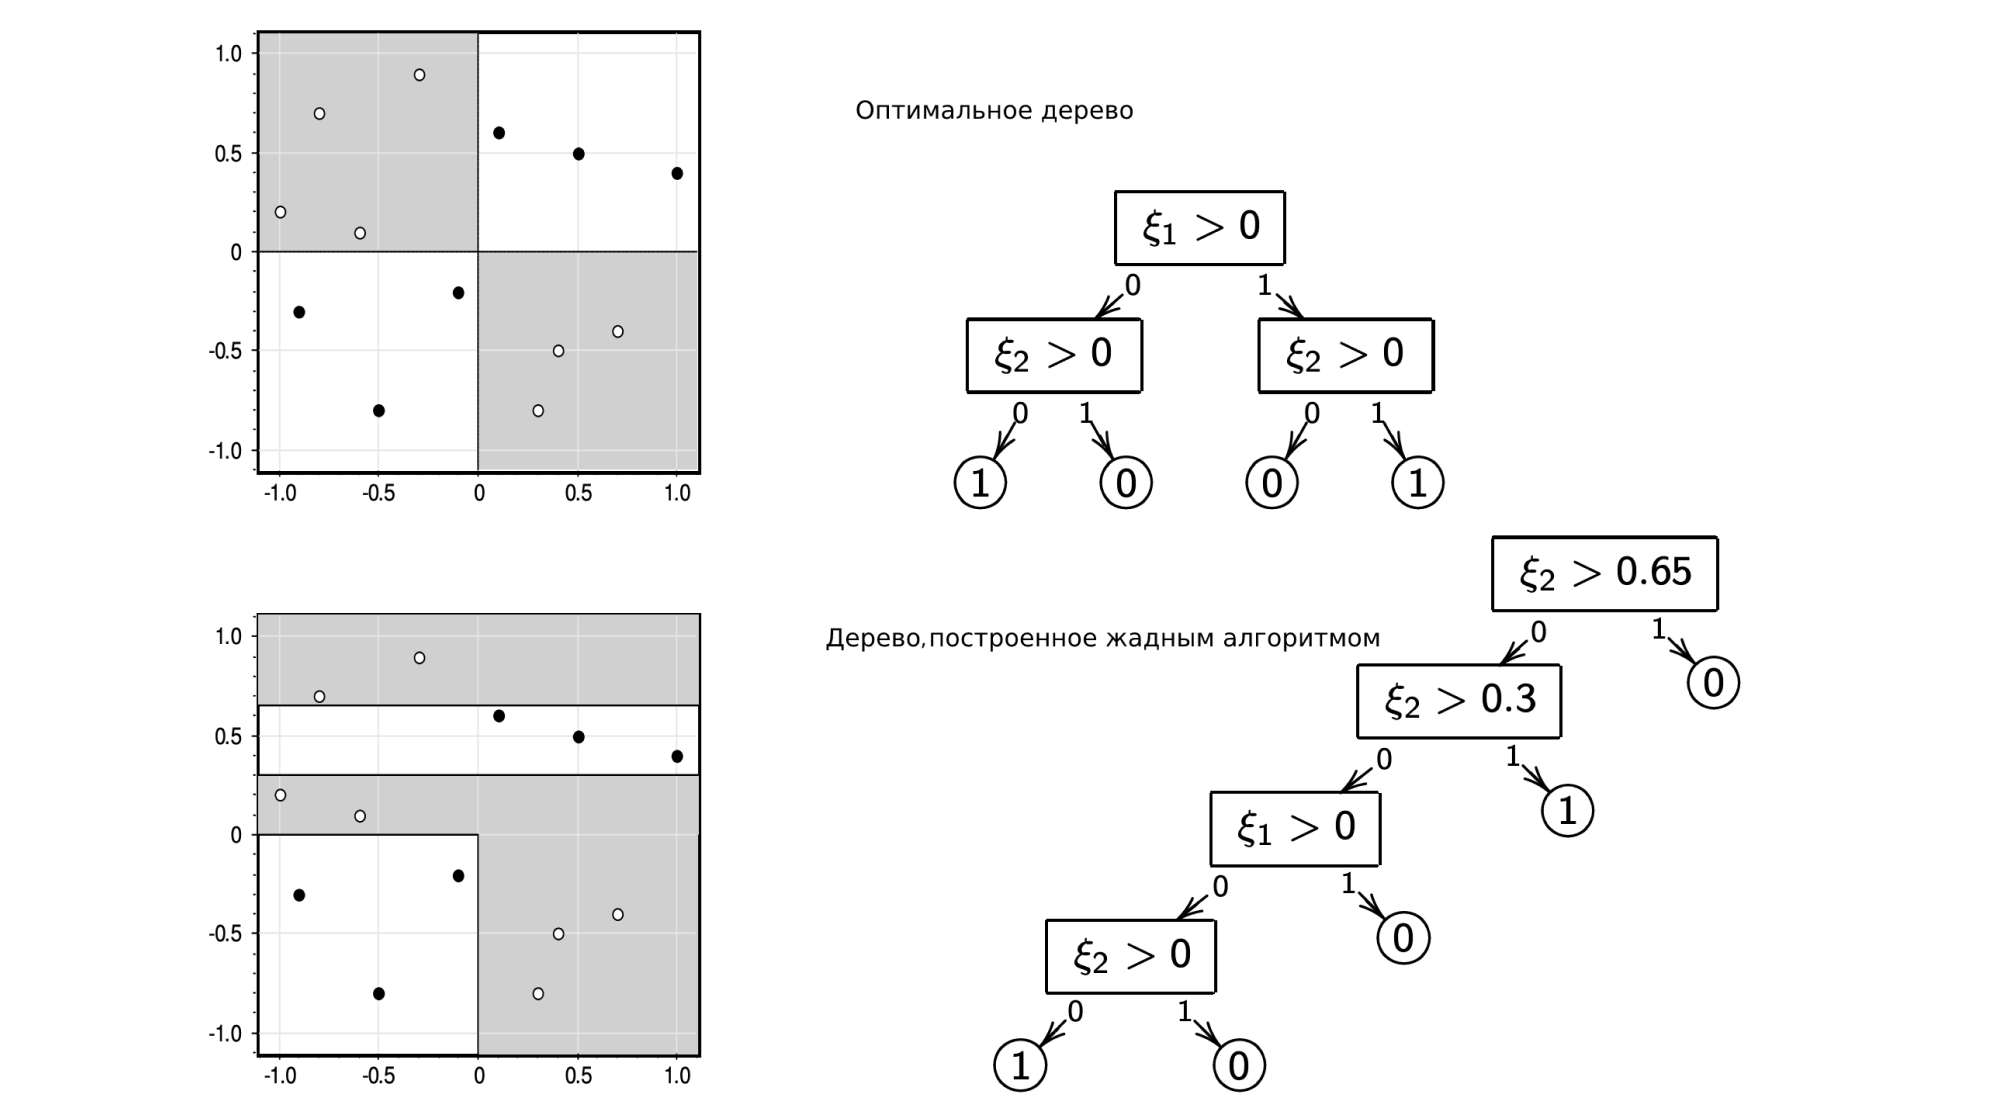
\includegraphics[width=\textwidth]{des-tree.png}
    \caption{Иллюстрация неоптимальности разбиения решающего дерева \cite{SHAD-trees}}
\end{figure}

Для того, чтобы избежать переобучения дерева (ситуации, когда обобщающая способность классификатора начинает падать из-за слишком хорошей точности на обучающей выборке), в данной работе ограничивалась глубина дерева.

\subsubsection{Градиентный бустниг. Gradient boosting}
Кратко опишем идею, стоящую за градиентным бустингом (В данной работе говорится именно о GBDT, т.е. градиентном бустинге, построенном на решающих деревьях). Эта модель хорошо показывает себя на неоднородных данных, т.е. данных, представимых в виде набора признаков, таблицы и способен хорошо находить и приближать нелинейные зависимости. Идея градиентного бустинга проста: будем использовать ансамбль простых моделей, каждая из которых плохо приближает истинную зависимость, чтобы давать предсказания. Причем каждая последующая модель в ансамбле добавляется так, чтобы уменьшить ошибку уже имеющегося ансамбля. Теперь более формально. Для решения будем строить композицию из $K$ базовых алгоритмов (в нашем случае - деревьев):

\[ a(x)= a_K(x) = b_1(x) + b_2(x) + ... + b_K(x) \]

При дальнейшем построении используется следующая идея: при обучении одного дерева $b_1(x)$ нам известны объекты, на которых его предсказание было неверным. Тогда мы можем обучить следующее дерево $b_2(x)$ предсказывать разницу $s_i^1 = y_i - b_1(x_i) = y_i - a_1(x_i)$ между результатами первого дерева и истинной зависимостью для каждого объекта обучающей выборки. Данная разница выражается через градиент функции потерь:
\[ s_i^k = y_i - a_1(x_i) = -\dfrac{\partial L(y_i, z)}{\partial z} |_{z = a_1(x_i)} \]

Или, в общем случае:

\[ s_i^k = y_i - a_k(x_i) = -\dfrac{\partial L(y_i, z)}{\partial z} |_{z = a_k(x_i)} \]
Поэтому бустинг и называется градиентным. Аналогично будет обучено третье дерево и т.д. На каждом $k$-м шаге вычисляется разница между целевой переменной и предсказанием композиции $k - 1$ алгоритмов, после чего $k$-е дерево учится предсказывать эту разницу, после чего композиция $a(x)$ обновляется:

\[ a_k(x) = a_{k-1}(x) + b_k(x) \]

Обучение K базовых алгоритмов завершает построение композиции и обучение модели.


\newpage %% Исследование и построение решения задачи
\chapter{Описание практической части}
\label{sec:Chapter4} \index{Chapter4}
Если в рамках работы писался какой-то код, здесь должно быть его описание: выбранный язык и библиотеки и мотивы выбора, архитектура, схема функционирования, теоретическая сложность алгоритма, характеристики функционирования (скорость/память).

\section{Структура проекта}

\section{Пример работы}

\newpage %% Описание практической части
\section{Заключение}
\label{sec:Chapter5} \index{Chapter5}

В результате данной работы:
\begin{itemize}
    \item Был создан классификатор сообщений предупреждений статического анализатора на два класса: true positive и false positive. Полученный классификатор позволяет приоритизировать предупреждения, т.к. помимо предсказания может указывать еще и уверенность в нем. Классификатор показал высокий precision (95 и 98\% для decision tree и GBDT соответственно) и приемлемый recall (88 и 94\%) на тестовой выборке. Также, классификатор на основе модели градиентного бустинга показал лучшую обобщаюцую способность, корректно отработав на представленных реальных примерах. На большую гибкость модели градиентного бустинга в данной задаче указывает еще и высокие (по сравнению с решающим деревом) precision и recall.
    \item Был рассмотрен метод генерации датасета при помощи тестовых сюит для статических анализаторов. Рассмотренный метод был реализован и использован для обучения вышеописанных моделей. Удалось найти набор признаков, время на извлечение которых значительно быстрее времени компиляции проекта и не требует его сборки. Это является большим плюсом, т.к. для языков C/C++ процесс сборки может быть сложным и не является стандартизованным. Поэтому возможность извлекать признаки из отдельных файлов очень полезна и заметно упрощает генерацию датасета на произвольной кодовой базе.
    \item Было обсуждено, как полученные в результате обучения модели могут быть полезны при разработке и поддержке статических анализаторов разработчиками.
\end{itemize}

В ходе работы большинство поставленных задач было реализовано. Также был обозначен фронт будущих работ, нацеленных на улучшение полученного результата и исправление всех обозначенных в процессе работы минусов.

\newpage %% Заключение

%% Don't change the following lines
\nocite{*}
% \bibliography{references}
% \printbibliography
\printbibliography[heading=bibintoc, title={Список литературы}]

%% в зависимости от надобности подключаем раздел "Приложениие"
% \newpage
% \section{Приложение}
\addcontentsline{toc}{section}{Приложение}
\label{sec:Apendix} \index{Apendix}

Здесь необходимо написать приложение, которое вы должны придумать самомтоятельно
\end{document}